% Included from both -slides and -handout versions.

\mode<presentation>
{
  \usetheme{default}
  \useoutertheme{infolines}
}

\usepackage[english]{babel}
\usepackage[latin1]{inputenc}
\usepackage{graphicx}
\usepackage{times}
\usepackage[T1]{fontenc}
\usepackage{fancyvrb}
\usepackage{hyperref}
\usepackage{listings}
\begin{document}
\lstset{language=C, escapeinside={(*@}{@*)}, numbers=left,
  basicstyle=\tiny, showspaces=false, showtabs=false}

\def\Tiny{\fontsize{4pt}{4pt} \selectfont}

\title{L41: Lab 4 - The TCP State Machine}
\author{Dr Robert N. M. Watson}
\date{25 January 2016}

\begin{frame}
  \titlepage
\end{frame}

\section{Introduction}

\begin{frame}
  \frametitle{L41: Lab 4 - The TCP State Machine}

  \begin{itemize}
    \item The TCP state machine
    \item TCP-socket mode for IPC benchmark mode
    \item DTrace probes of interest
  \end{itemize}
\end{frame}

\begin{frame}[fragile]
  \frametitle{Lect 6: The Transmission Control Protocol (TCP)}

  \begin{columns}[T]
    \column{0.45\textwidth}

  \begin{Tiny}
    \begin{verbatim}
September 1981                             Transmission Control Protocol
                                                Functional Specification

                              +---------+ ---------\      active OPEN  
                              |  CLOSED |            \    -----------  
                              +---------+<---------\   \   create TCB  
                                |     ^              \   \  snd SYN    
                   passive OPEN |     |   CLOSE        \   \           
                   ------------ |     | ----------       \   \         
                    create TCB  |     | delete TCB         \   \       
                                V     |                      \   \     
                              +---------+            CLOSE    |    \   
                              |  LISTEN |          ---------- |     |  
                              +---------+          delete TCB |     |  
                   rcv SYN      |     |     SEND              |     |  
                  -----------   |     |    -------            |     V  
 +---------+      snd SYN,ACK  /       \   snd SYN          +---------+
 |         |<-----------------           ------------------>|         |
 |   SYN   |                    rcv SYN                     |   SYN   |
 |   RCVD  |<-----------------------------------------------|   SENT  |
 |         |                    snd ACK                     |         |
 |         |------------------           -------------------|         |
 +---------+   rcv ACK of SYN  \       /  rcv SYN,ACK       +---------+
   |           --------------   |     |   -----------                  
   |                  x         |     |     snd ACK                    
   |                            V     V                                
   |  CLOSE                   +---------+                              
   | -------                  |  ESTAB  |                              
   | snd FIN                  +---------+                              
   |                   CLOSE    |     |    rcv FIN                     
   V                  -------   |     |    -------                     
 +---------+          snd FIN  /       \   snd ACK          +---------+
 |  FIN    |<-----------------           ------------------>|  CLOSE  |
 | WAIT-1  |------------------                              |   WAIT  |
 +---------+          rcv FIN  \                            +---------+
   | rcv ACK of FIN   -------   |                            CLOSE  |  
   | --------------   snd ACK   |                           ------- |  
   V        x                   V                           snd FIN V  
 +---------+                  +---------+                   +---------+
 |FINWAIT-2|                  | CLOSING |                   | LAST-ACK|
 +---------+                  +---------+                   +---------+
   |                rcv ACK of FIN |                 rcv ACK of FIN |  
   |  rcv FIN       -------------- |    Timeout=2MSL -------------- |  
   |  -------              x       V    ------------        x       V  
    \ snd ACK                 +---------+delete TCB         +---------+
     ------------------------>|TIME WAIT|------------------>| CLOSED  |
                              +---------+                   +---------+

                      TCP Connection State Diagram
                               Figure 6.
\end{verbatim}
  \end{Tiny}

    \column{0.45\textwidth}
    \bigskip
    \begin{itemize}
      \item V. Cerf, K. Dalal, and C. Sunshine, \textit{Transmission Control
	Protocol (version 1)}, INWG General Note \#72, December 1974.
      \item In practice: Jon Postel, Ed, \textit{Transmission Control
	Protocol: Protocol Specification}, RFC 793, September, 1981.
    \end{itemize}
  \end{columns}

\end{frame}

\begin{frame}
  \frametitle{Lect 6: TCP goals and properties}

  \begin{columns}[T]
    \column{0.38\textwidth}
      \smallskip
      \begin{center}
	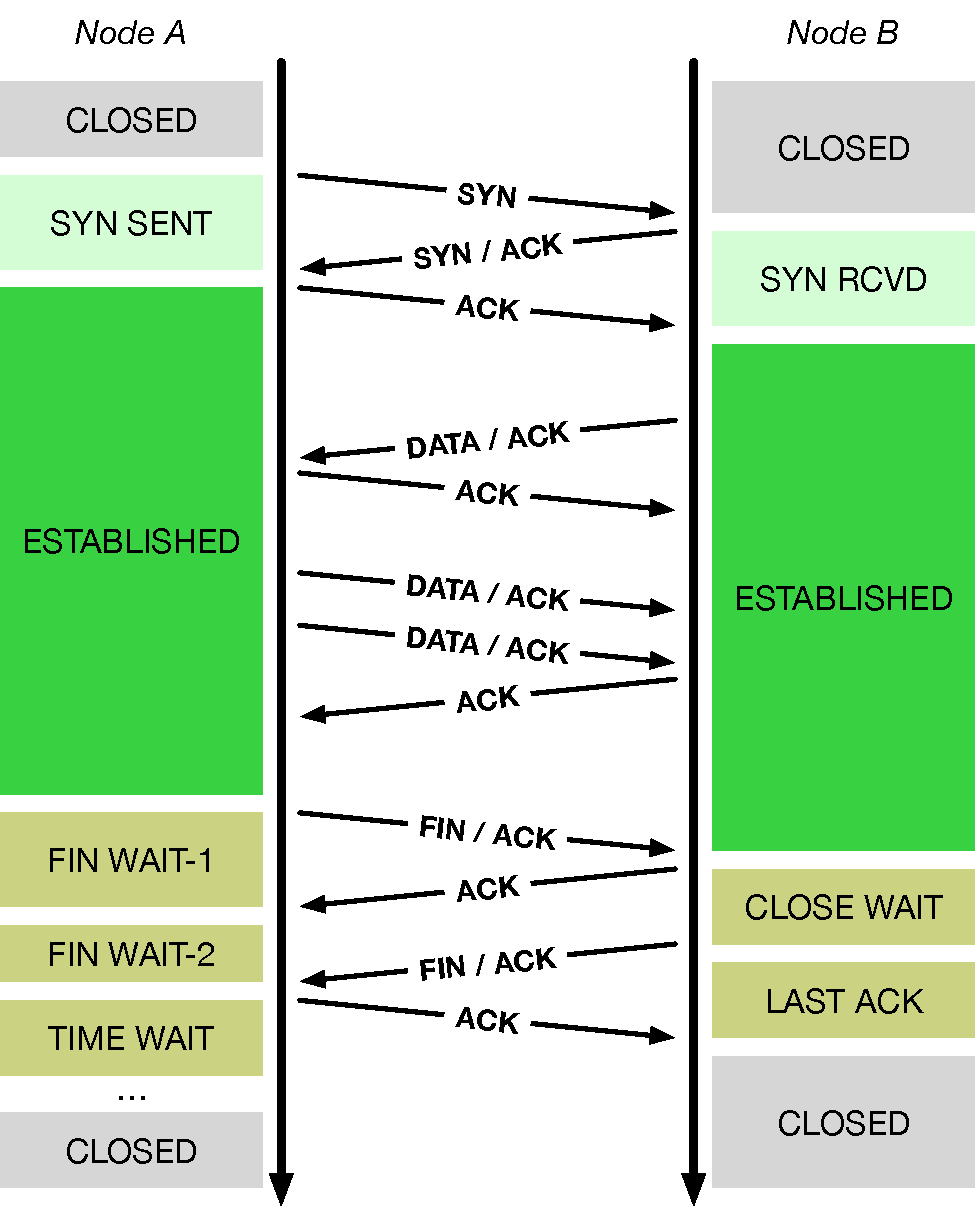
\includegraphics[width=1.15\textwidth]{../../figures/tcp-timeline.pdf}
      \end{center}

    \column{0.52\textwidth}
      \begin{itemize}
	\item Reliable, ordered, byte-stream transport protocol over IP
	%\item Connections identified by unique IP-port 4-tuple
	\item Three-way handshake: SYN~/ SYN-ACK~/ ACK (mostly!)
        \item Flow control via advertised window size in ACKs
	\item Congestion control via packet loss and ECN (`fairness')

	\pause

	\item Network may delay, (reorder), drop, corrupt packets
	\item Sequence numbers ACK'd; data retransmitted on loss
	\item Round-Trip Time (RTT) measured to time out loss

	%\pause

	%\item Complex teardown permits `half-close' and port reuse
      \end{itemize}

  \end{columns}
\end{frame}

\begin{frame}[fragile]
  \frametitle{Loopback interface, IPFW, and DUMMYNET}

  \begin{itemize}
    \item Loopback interface
    \begin{itemize}
      \item Simulated local network interface: packets ``loop back''
      \item Interface name \texttt{lo0}
      \item Assigned IPv4 address 127.0.0.1
      \item Configure the loopback MTU once per boot.
    \end{itemize}

    \pause

    \item IPFW - IP firewall by Rizzo, et al.
    \begin{itemize}
      \item Numbered rules classify packets and perform actions
      \item Actions include accept, reject, inject into DUMMYNET ...
      \item We will match lab flows using the TCP port number 10,141
      \item Configure \textbf{once per boot} (and with care!)
    \end{itemize}

    \pause

    \item DUMMYNET - link simulation tool by Rizzo, et al.
    \begin{itemize}
      \item Widely used in network research
      \item Impose simulated network conditions -- delay, bandwidth, loss, ...
      \item Configure and reconfigure as needed for experiments
    \end{itemize}
    \item Instructions in lab assignment
  \end{itemize}
\end{frame}

\begin{frame}[fragile]
  \frametitle{TCP in the IPC benchmark}

  \begin{tiny}
    \begin{verbatim}
root@beaglebone:/data/ipc # ./ipc-static 
ipc-static [-Bqsv] [-b buffersize] [-i pipe|local|tcp] [-p tcp_port]
        [-P l1d|l1i|l2|mem|tlb|axi] [-t totalsize] mode

Modes (pick one - default 1thread):
    1thread                IPC within a single thread
    2thread                IPC between two threads in one process
    2proc                  IPC between two threads in two different processes

Optional flags:
    -B                     Run in bare mode: no preparatory activities
    -i pipe|local|tcp      Select pipe, local sockets, or TCP (default: pipe)
    -p tcp_port            Set TCP port number (default: 10141)
    -P l1d|l1i|l2|mem|tlb|axi  Enable hardware performance counters
    -q                     Just run the benchmark, don't print stuff out
    -s                     Set send/receive socket-buffer sizes to buffersize
    -v                     Provide a verbose benchmark description
    -b buffersize          Specify a buffer size (default: 131072)
    -t totalsize           Specify total I/O size (default: 16777216)
\end{verbatim}
  \end{tiny}

  \begin{itemize}
    \item \texttt{tcp} IPC type
    \item \texttt{-p} argument to set the port number
  \end{itemize}
\end{frame}

\begin{frame}
  \frametitle{DTrace probes}

  Described in more detail in the lab assignment:

  \medskip

  \begin{description}
    \item[fbt::syncache\_add:entry] TCP segment installs new SYN-cache entry
    \item[fbt::syncache\_expand:entry] TCP segment converts SYN-cache entry to
      full connection
    \item[fbt::tcp\_do\_segment:entry] TCP segment received post-SYN cache
    \item[fbt::tcp\_state\_change:entry] TCP state transition
  \end{description}

  \medskip

  \begin{scriptsize}
    We are using implementation-specific probes (FBT) rather than portable TCP
    probes due to a bug in the FreeBSD/armv7 implementation of DTrace -- the
    last (and most critical!) argument goes missing: the TCP header!  We will
    fix this .. but not today.
  \end{scriptsize}
\end{frame}

\begin{frame}
  \frametitle{Exploratory questions}

  \begin{itemize}
    \item Trace state transitions occurring in test TCP connections
    \item Identify causes of transitions -- packets, system calls (etc)
    \item Varying one-way latency, explore performance of the benchmark with
      TCP
  \end{itemize}
\end{frame}

\begin{frame}
  \frametitle{Experimental questions for the lab report}

  \begin{itemize}
    \item Plot a TCP state-transition diagram for both directions of a flow
    \item Label the state-transition diagram with causes
    \item Compare the diagram with RFC 793
    \item Begin performance analysis of TCP latency vs. throughput
  \end{itemize}

  \medskip

  In the next lab, we will start a causal analysis of why latency affects
  bandwidth in the way that it does
\end{frame}

\begin{frame}
  \frametitle{This lab session}

  \begin{itemize}
    \item Set up IPFW, DUMMYNET, and loopback MTU (see notes)
    \item Ask us if you have any questions or need help
    \item Start with the TCP state machine analysis
  \end{itemize}
\end{frame}

\end{document}
